\documentclass[12pt,preprint]{aastex}
\usepackage{amssymb,amsmath}
%\usepackage{color,hyperref}
%\definecolor{linkcolor}{rgb}{0,0,0.25}
%\hypersetup{
%  colorlinks=true,        % false: boxed links; true: colored links
%  linkcolor=linkcolor,    % color of internal links
%  citecolor=linkcolor,    % color of links to bibliography
%  filecolor=linkcolor,    % color of file links
%  urlcolor=linkcolor      % color of external links
%}
\setlength{\emergencystretch}{2em}%No overflowing references
\newcommand{\ie}{i.e.}
\newcommand{\etal}{et al.}
\newcommand{\eg}{e.g.}
\newcommand{\eqnname}{equation}
\newcommand{\figurenames}{\figurename s}
\newcommand{\sectionname}{$\mathsection$}
\newcommand{\tvector}[1]{\boldsymbol{\vec{#1}}}
\newcommand{\vx}{\tvector{x}}
\newcommand{\vv}{\tvector{v}}
\newcommand{\Gaia}{\emph{Gaia}}
\newcommand{\apogee}{APOGEE}
\newcommand{\vR}{\ensuremath{v_R}}
\newcommand{\vphi}{\ensuremath{v_{\phi}}}
\newcommand{\vo}{\ensuremath{v_0}}
\newcommand{\Ro}{\ensuremath{R_0}}
\newcommand{\ro}{\Ro}

\begin{document}

\title{Tracing the Hercules stream around the Galaxy}
\author{Jo~Bovy}%\altaffilmark{1,2}}
\affil{Center for Cosmology and Particle Physics, Department of Physics, New York University, 4 Washington Place, New York, NY 10003, USA}
\email{jb2777@nyu.edu}
%\altaffiltext{1}{Center for Cosmology and Particle Physics, Department of Physics,
%  New York University, 4 Washington Place, New York, NY 10003, USA}
%\altaffiltext{2}{Correspondence should be addressed to jo.bovy@nyu.edu~.}

\begin{abstract}
It has been proposed that the Hercules stream, a group of co-moving
stars in the Solar neighborhood offset from the bulk of the velocity
distribution, is the result of resonant interactions between stars in
the outer disk and the Galactic bar. Only seen so far in the immediate
Solar neighborhood, I predict the distribution of stellar velocities
and the run of the Hercules stream as a function of location in the
Galactic disk in a simple model for the Galaxy and the bar that
produces the observed Hercules stream. I further show that the
Hercules feature is strong enough that it can be unambiguously
detected in the distribution of line-of-sight velocities in selected
directions. I quantify the most promising lines-of-sight for detection
in radial velocities: The most promising directions to target are at
$l \gtrsim 250^{\circ}$. The predictions presented here are only
weakly affected by distance uncertainties, assumptions about the
distribution function of the old stellar disk, and the details of the
Galactic potential including the effect of spiral structure;
\Gaia\ and future spectroscopic surveys of the Galactic disk will be
able to robustly test the origin of the Hercules stream and constrain
the properties of the Galactic bar.
\end{abstract}

\keywords{Galaxy: bulge --- Galaxy: disk --- Galaxy: evolution ---
  Galaxy: fundamental parameters --- Galaxy: kinematics and dynamics
  --- Galaxy: structure }

\section{Introduction}


baryon acoustic feature, coincidence problem

\section{Methodology}

We follow Dehnen's approach \citep{dehnen00a}. Only planar.


\section{Two-dimensional velocity distributions}


\section{The line-of-sight velocity distribution}


\section{Discussion}

\subsection{\Gaia}

\subsection{Radial velocity surveys}

SDSS-III Project Description\footnote{Available at
  \url{http://sdss3.org/collaboration/description.pdf}~.}

\acknowledgements David Hogg, Michael Blanton.

\begin{thebibliography}{}

%\bibitem[{{Binney} \& {Tremaine}(2008)}]{binneytremaine}
%{Binney},~J. \& {Tremaine},~S., 2008, {Galactic Dynamics: Second Edition}
%  (Princeton University Press)

\bibitem[Bailer-Jones(2008)]{bailerjones08a}
  Bailer-Jones, ~C.~A.~L., 2008,
  in IAU Symp.~254, ed.~J.~Andersen, J.~Bland-Hawthorn, and B.~Nordstr\"{o}m, (Dordrecht: Kluwer), 475  

\bibitem[Bensby \etal(2007)]{Bensby07a}
  Bensby,~T., \etal, 2007,
  \apjl, 655, L89

\bibitem[Blaauw(1970)]{Blaauw70a}
  Blaauw,~A., 1970, in IAU Symp.~38, ed.~W.~Becker \& I.~Kontopoulos (Dordrecht: Reidel), 199

\bibitem[Blitz \& Spergel(1991)]{blitz91a}
  Blitz,~L.~\& Spergel,~D.~N., 1991, \apj, 379, 631

\bibitem[Binney, Gerhard, \& Spergel(1997)]{binney97a}
  Binney,~J.~J., Gerhard,~O., \& Spergel,~D.~N., 1997,
  \mnras, 288, 365

\bibitem[Bissantz \& Gerhard(2002)]{bissantz02a}
  Bissantz,~N.~\& Gerhard,~O., 2002,
  \mnras, 330, 591

\bibitem[Bovy, Hogg, \& Roweis(2009)]{Bovy09a} Bovy,~J., Hogg,~D.~W., \& Roweis,~S.~T., 2009,
  \apj, 700, 1794

\bibitem[Bovy \& Hogg(2010)]{Bovy10a} Bovy,~J.~\& Hogg,~D.~W., 2010,
  \apj, in press

\bibitem[Caloi \etal(1999)]{caloi99a}
  Caloi,~V.~, \etal, 1999,
  \aap, 351, 925

\bibitem[Cole \& Weinberg(2002)]{cole02a}
  Cole,~A.~A.~\& Weinberg,~M.~D., 2002,
  \apjl, 574, L43

\bibitem[{{Dehnen}(1998)}]{Dehnen98b}
Dehnen,~W., 1998, \aj, 115, 2384

\bibitem[Dehnen(1999a)]{dehnen99a}
  Dehnen,~W., 1999a, \aj, 118, 1190

\bibitem[Dehnen(1999b)]{dehnen99b}
  Dehnen,~W., 1999b, \aj, 118, 1201

\bibitem[Dehnen(1999c)]{dehnen99c}
  Dehnen,~W., 1999c, \apj, 524, L35

\bibitem[Dehnen(2000)]{dehnen00a}
  Dehnen,~W., 2000, \aj, 119, 800

\bibitem[Fux(2001)]{fux01a}
  Fux,~R., 2001,
  \aap, 373, 511

\bibitem[Gardner \& Flynn(2010)]{gardner10a}
  Gardner,~E.~\& Flynn,~C., 2010,
  \mnras, in press

\bibitem[H\"{a}fner \etal(2000)]{hafner00}
  H\"{a}fner,~R., \etal, 2000,
  \mnras, 314, 433

\bibitem[Minchev \& Famaey(2009)]{minchev09a}
  Minchev,~I.~\& Famaey,~B., 2009,
  \apj L, submitted

\bibitem[Raboud \etal(1998)]{raboud98a}
  Raboud,~D., \etal, 1998,
  \aap, 335, L61

\bibitem[Shen \etal(2010)]{Shen10a}
  Shen,~J., \etal, 2010, \apj L, submitted

\bibitem[Sellwood \& Binney(2002)]{sellwood02a}
  Sellwood,~J.~A.~\& Binney,~J.J., 2002,
  \mnras, 336, 785

\bibitem[Shu(1969)]{shu69a}
  Shu,~F.~H., 1969,
  \apj, 158, 505

\bibitem[Skuljan, Hearnshaw, \& Cottrell(1999)]{Skuljan99a}
  Skuljan,~J., Hearnshaw,~J.~B., \& Cottrell,~P.~L., 1999, \mnras, 308, 731

\end{thebibliography}


\clearpage
\begin{figure}
\includegraphics[width=0.5\textwidth]{veldist.eps}
\caption{The velocity distribution of nearby ($\lesssim 100$ pc) stars
  from \citet{Bovy09a}. The Hercules moving group is visible as an
  overdensity at \vphi $\approx$ -0.2 $\vo$.}\label{fig:obs}
\end{figure}

\clearpage
\begin{figure}
\includegraphics[width=\textwidth]{rphi2d.ps}
\caption{Two-dimensional velocity distributions along the Solar
  circle. The axes of each subpanel are the radial and tangential
  velocities in Galactocentric cylindrical coordinates for the same
  ranges as in \figurename~\ref{fig:obs}. The velocity distributions
  on the other side of the Galaxy are obtained by shifting the
  azimuths by 180$^{\circ}$. }\label{fig:rphi2d}
\end{figure}

\clearpage
\begin{figure}
\includegraphics[width=\textwidth]{rphi1d.ps}\\
\includegraphics[width=\textwidth]{rphi1d2.ps}
\caption{Line-of-sight velocity distributions along the Solar
  circle. The range in line-of-sight velocities in each subpanel is as
  in \figurename~\ref{fig:1dvar}. The gray curve in each panel is the
  predicted distribution for an axisymmetric, steady-state
  Galaxy.}\label{fig:rphi1d}
\end{figure}

\clearpage
\begin{figure}
\includegraphics[width=0.5\textwidth]{detecta.ps}
\includegraphics[width=0.5\textwidth]{detectb.ps}
\caption{Kullback-Leibler divergence between the predicted
  line-of-sight velocity distributions with and without the
  bar. Darker values have a larger discriminatory potential. The left
  panel uses the full line-of-sight velocity distributions, the right
  panel excludes the main mode of the velocity distribution that is
  likely to be affected by other dynamical and phase-space
  effects. The concentric dashed lines indicate
  constant-distance slices from the Sun, starting at 1 kpc and spaced
  2 kpc apart.  The white dashed lines indicate the boundaries of the
  four quadrants in Galactic longitude.  The white dashed-dotted line
  shows the region of the sky that \apogee\ can see (-5$^{\circ} \leq
  l \leq 250^{\circ}$).}\label{fig:detect}
\end{figure}

\clearpage
\begin{figure}
\includegraphics[width=0.5\textwidth]{distuncertain.ps}
\includegraphics[width=0.5\textwidth]{df.ps}\\
\includegraphics[width=0.5\textwidth]{slope.ps}
\includegraphics[width=0.5\textwidth]{barstrength.ps}
\caption{Variation of the predicted velocity distribution at R = 1.075
  \Ro , $\phi = -21^{\circ}$ (d= 0.4 \Ro, $l$ = 270$^{\circ}$) with
  distance uncertainties, parameters and shape of the distribution
  function, slope of the rotation curve, and bar
  strength.}\label{fig:1dvar}
\end{figure}



\end{document}
